% !TeX root = ../../navier-stokes-manuscript.tex
\begin{center}
\captionsetup{hypcap=false}
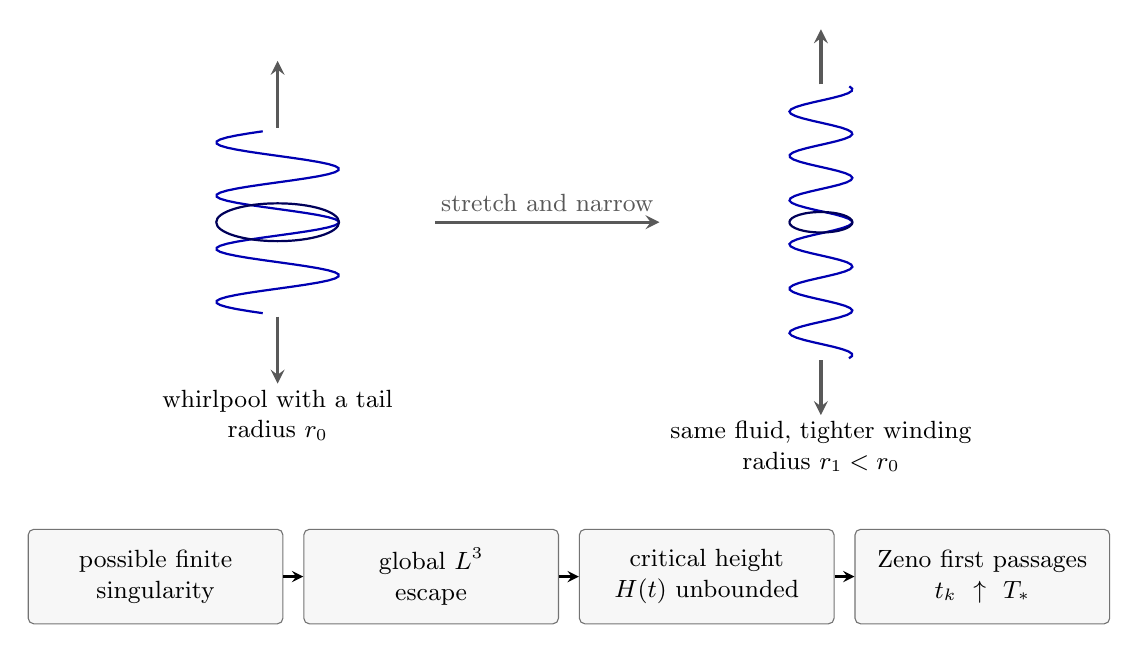
\begin{tikzpicture}[
  >=stealth,
  logic/.style={draw=black!55,rounded corners=2pt,fill=black!3,
    align=center,text width=3.0cm,minimum height=1.2cm,font=\small},
  note/.style={align=center,font=\small}
]
  \draw[blue!70!black,thick,domain=-1.1:1.1,samples=90]
    plot ({-3.7+0.78*cos(560*\x)},{1.05*\x+2.4});
  \draw[blue!35!black,thick]
    (-4.48,2.4) arc[start angle=180,end angle=540,x radius=.78,y radius=.24];
  \draw[->,very thick,black!65] (-3.7,3.6)--(-3.7,4.45);
  \draw[->,very thick,black!65] (-3.7,1.2)--(-3.7,.35);
  \node[note] at (-3.7,-.05) {whirlpool with a tail\\radius \(r_0\)};

  \draw[->,very thick,black!65]
    (-1.7,2.4)--(1.15,2.4)
    node[midway,above,note] {stretch and narrow};

  \draw[blue!70!black,thick,domain=-1.35:1.35,samples=120]
    plot ({3.2+0.40*cos(820*\x)},{1.28*\x+2.4});
  \draw[blue!35!black,thick]
    (2.80,2.4) arc[start angle=180,end angle=540,x radius=.40,y radius=.13];
  \draw[->,very thick,black!65] (3.2,4.15)--(3.2,4.85);
  \draw[->,very thick,black!65] (3.2,.65)--(3.2,-.05);
  \node[note] at (3.2,-.45) {same fluid, tighter winding\\radius \(r_1<r_0\)};

  \node[logic] (a) at (-5.25,-2.1) {possible finite\\singularity};
  \node[logic] (b) at (-1.75,-2.1) {global \(L^3\)\\escape};
  \node[logic] (c) at (1.75,-2.1) {critical height\\\(H(t)\) unbounded};
  \node[logic] (d) at (5.25,-2.1) {Zeno first passages\\\(t_k\uparrow T_*\)};
  \draw[->,thick] (a)--(b);
  \draw[->,thick] (b)--(c);
  \draw[->,thick] (c)--(d);
\end{tikzpicture}
\captionof{figure}{The perfectly stretching vortex keeps one physical danger in view while the implication chain below it moves to global quantities.}
\label{fig:BalancedVortexCriticalRoute}
\end{center}
